\chapter{Testing}

The whole system has many components and it is a widely accepted fact that the more complex the system is, the more prone to errors and bugs it is. In this chapter I will describe the benchmarking tests I performed on the most complex part - the tracking engine - and the user tests I performed not only on the front-end applications but also on the whole workflow of the system as well.

\section{Benchmark Tests}

To verify that the Tracking Engine handles an extensive load it is important to simulate a real-world peak that could occur during everyday usage. I identified the biggest bottlenecks to be the client side (networking issues like poor EDGE connection) and the workers' parsing job (how big a task can they manage?). The Gateway server has an automatic load-balancer, so there shouldn't be a problem, just like with all other automatically scaled components by Amazon (S3 and SQS).

\subsection{Workers}

To verify how big a load a single worker can handle, I created data on the front-end of various sizes and sent it to the server. I turned on a logging system, CloudWatch, that told me the precise times when a job started on a worker and when it finished.

\begin{table}[!ht]
\begin{center}
\begin{tabular}{|c|c|c|c|}
\hline
\textbf{Number of entries} & \textbf{Execution Start} & \textbf{Execution End} & \textbf{Duration} \\
\hline
100 & 15:46:35.966 & 15:46:41.595 & $5.629s$ \\
\hline
500 & 16:06:57.851 & 16:07:15.265 & $17.414s$ \\
\hline
1000 & 15:51:23.311 & 15:51:59.060 & $35.749s$ \\
\hline
5000 & N/A & N/A & N/A \\
\hline
10000 & N/A & N/A & N/A \\
\hline
\end{tabular}
\end{center}
\caption{Worker Processing Times}
\label{tab:table_worker}
\end{table}

\newpage

To give it a visual perspective:

\begin{figure}[!ht]
\begin{center}
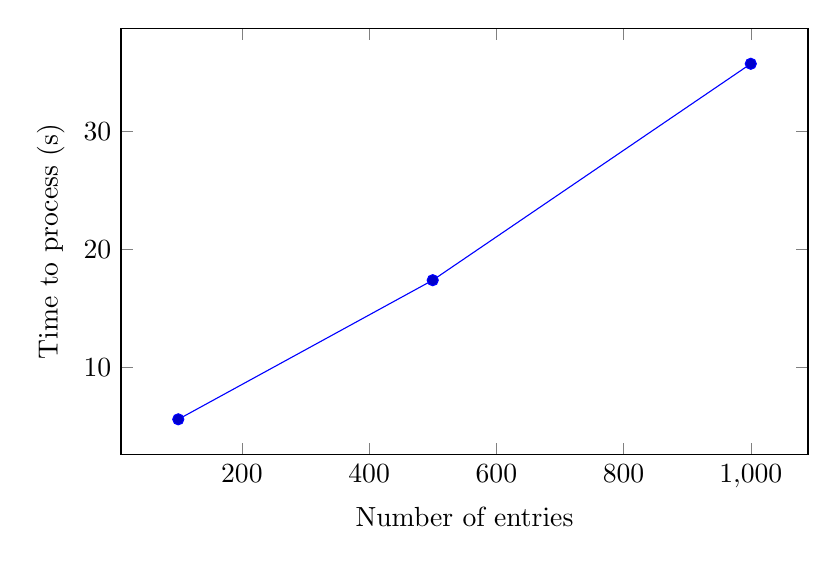
\begin{tikzpicture}
    \begin{axis}[
    		height=7cm,
		width=0.85\textwidth,
		xlabel={Number of entries},
    		ylabel={Time to process (s)}
    	]
    \addplot coordinates { 
    		(100, 5.629) 
    		(500, 17.414) 
    		(1000, 35.749)};
    \end{axis}
\end{tikzpicture}
\end{center}
\caption{Worker Processing Times Graph}
\end{figure}

The graph itself doesn't show anything that would be out of the ordinary, so why did the workers fail to process 5000 and 10000 entries? The scenario of what actually happened is interesting in both cases and it isn't the fault of the workers themselves:

\begin{enumerate}
	\item {\bf 5000 entries: } When the first worker got the message to handle 5000 entries sitting on S3, he reached out for them and started parsing. However he did not make it in the given time of message execution and therefore the message was marked as failed. When the SQS tried to deliver it again, the worker was still processing the data and so it was sent to another worker, who started parsing them. Then finally the first worker returned "200 OK" which resulted in an inconsistent state and the whole system went into "Warning". CloudWatch stopped the servers and I couldn't get the execution times. The result was that, unfortunately, the data in the database was saved twice.
	\item {\bf 10000 entries: } In the last round, it simply took too long and the whole worker crashed and so did the second one soon after the first one.
\end{enumerate}

\subsubsection*{Conclusion}

Even though compression does save some data on the client side, it also introduces a new complexity on the server side that is very hard to parallelize, so it is important to find a "good enough" amount of entries to be uploaded in a single batch report.

\newpage

\subsection{Client-side Compression Rate}

To continue the search for optimum load on both sides, I measured the performance of the GZIP compression library. I performed it on a real device (iPhone 6S), using logging capabilities in Xcode. 

\begin{table}[!ht]
\begin{center}
\begin{tabular}{|c|c|c|c|}
\hline
\textbf{Number of entries} & \textbf{Before compression} & \textbf{After compression} & \textbf{Compression rate} \\
\hline
100 & 51.41kB & 0.67kB & 76.7x \\
\hline
500 & 252.98kB & 1.65kB & 153.3x \\
\hline
1000 & 504.92kB & 2.87kB & 177.8x \\
\hline
5000 & 2520.55kB & 12.65kB & 199.3x \\
\hline
10000 & 5040.08kB & 24.89kB & 202.5x \\
\hline
\end{tabular}
\end{center}
\caption{Client-side Compression Rate}
\label{tab:compression}
\end{table}

To give it a visual perspective:

\begin{figure}[!ht]
\begin{center}
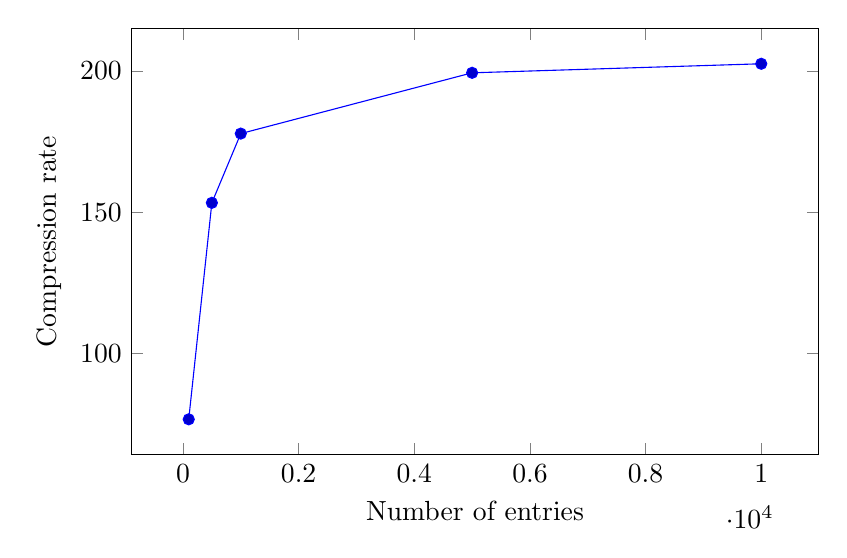
\begin{tikzpicture}
    \begin{axis}[
    		height=7cm,
		width=0.85\textwidth,
		xlabel={Number of entries},
    		ylabel={Compression rate}
    	]
    \addplot coordinates { 
    		(100, 76.7) 
    		(500, 153.3) 
    		(1000, 177.8) 
    		(5000, 199.3) 
    		(10000, 202.5)};
    \end{axis}
\end{tikzpicture}
\end{center}
\caption{Compression Rate Graph}
\end{figure}

I was quite surprised by the performance, even though I expected it to be performing very well, given the fact that the JSON file structure is very repetitive. What I was equally suprised by was the logarithmic shape of the curve. In other words, I did not expect the compression rate to slow down.

\subsubsection*{Conclusion}

The best amount seems to be somewhere in the range 400 - 700 entries. Combined with the knowledge from the previous measurement (worker processing time) I would aim to be in lower numbers, perhaps 400 - 600. That ensures a very good compression rate (\textasciitilde 150x) and also good processing time on the backend (\textasciitilde 18s)

\newpage

\section{User Tests}

I performed user tests in three different ways:

\begin{enumerate}
	\item Personal interviews
	\item Scenario test
	\item Panel discussion
\end{enumerate}

Each tested different aspects of the whole solution and each brought me some new insights into which problems I had overlooked during the development.

\subsection{Personal Interviews}

The personal interviews were held with three different people, each from a different department. I showed them the whole workflow and asked them to give me feedback on anything they wanted.

\subsubsection{Test Setup}

The interviews were held in a company kitchen - an area where people relax, chat and hang out during their personal breaks. The work was presented on a laptop (JIRA workflow and the deployment in the AWS console, should it be of any interest) and an iPhone 6S. Both devices were directly accessible to the person being interviewed.

I extracted the highlights from each interview:

\begin{enumerate}
		\item Associate Director, Applied Technology
		\begin{itemize}
				\item[] "I like the fact that I define the domain vocabulary once. Once and that's it. That's great."
				\item[] "Could we wire-up the installation IDs to the user IDs to ensure that 10 installations on the same device are counted as one?"
				\item[] (Looking at the Timeseries Application) "Yes! That's exactly what I want to see."
		\end{itemize}			
		
		\item Mobile Application Development Lead
		\begin{itemize}
				\item[] "I didn't quite understand the concept of WATCH when you first said it, maybe name it differently, like "Event" for example?"
				\item[] "Is it possible to produce a user flow? Like how the user moves throughout the application?"
				\item[] "How do you address a change in the configuration file? Is there a way to ensure I am not reporting something I was reporting before?"
				\item[] "How do you ensure that the content is sent later if it fails? Are you using operations.io or some other framework?"
		\end{itemize}
		
		\item UX Lead
		\begin{itemize}
				\item[] "Could you show me how I, as a UX designer, would use this? Would I use it only at the start or towards the end as well?"
				\item[] "Can I edit measurable items?"
				\item[] "So here, I would add "WATCH: Button Start in the header" and the programmer would receive it in his configuration file, right?" (a task a programmer would refer to as "Back button in a UINavigationBar")
		\end{itemize}
\end{enumerate}

The interviews were so fruitful; they validated the main idea as all three were very interested in the project and were asking how soon we could deploy it to test it. 

At the same time, they uncovered the questions I didn't ask myself, such as the configuration file versioning and change management.

And lastly, they brought up ideas for future development.

\subsection{Scenario Test}

The scenario test was performed on the administrative application, made for creating configuration files for developers to implement. The five people \cite{Nielsen:1993:MMF:169059.169166} I asked to test the application were from different departments and also different positions (technical support, assistant, programmer, etc.)

\subsubsection{Test Setup}

The test was performed on an iPhone 6S device, running the real application, connected to real data. Issues in JIRA were created by me, ready to be used during the test (there was no need for the testers to create those issues, because that is JIRA workflow, not the workflow of the application).

The test was carried out in a semi-informal environment - in the company library on a comfortable sofa, surrounded by bookshelves. I sat in front of the tester, not peeking over his/her shoulder. 

I asked each tester to narrate every step he/she made and point out any inconvenience, should one ever occur. I assured everybody that criticism was welcome and that there was absolutely no problem if they failed to perform the task. That was what the test was about and it was vital for the tester to be aware of that.

\newpage

\subsubsection{Scenario}

The scenario was made up of the following steps:

\begin{enumerate}
	\item Start creating a new configuration.
	\item The configuration should be made for the project "Semantic Analysis of User Interactions".
	\item Select to measure the performance of the measurement switch.
	\item Are there any special values to be tested?
	\item Generate and upload the configuration file to Dropbox.
	\item Can you tell me precisely what was in the configuration file again?
\end{enumerate}

The designed path to achieve these was:

\begin{enumerate}
	\item Click on the plus button in the top right-hand corner in the navigation bar.
	\item Scroll to letter "S" and select the project "Semantic Analysis of User Interactions".
	\item Click on the issue "Performance measurement switch".
	\item The correct answer is yes - it is written in the comment below the name of the issue. There are two watched values.
	\item Click done and then click on the button "Upload to Dropbox". Once you have clicking done after a successful upload, the application is automatically brought back to the first screen.
	\item Click on the button in the bottom right-hand corner "View Generated Configurations". Select the one with the most recent time by clicking on it and it leads directly to a list with all the issues in the configuration.
\end{enumerate}

\newpage

How the testers performed:

\begin{table}[!ht]
\begin{center}
\begin{tabular}{|c|c|c|c|c|c|}
\hline
\textbf{Step} & \textbf{Person 1} & \textbf{Person 2} & \textbf{Person 3} & \textbf{Person 4} & \textbf{Person 5} \\
\hline
\textbf{1.} & OK & OK & "I guess & OK & Tracked  \\
& & & this plus?" & & Applications \\
\hline
\textbf{2.} & OK & OK & OK & OK & OK \\
\hline
\textbf{3.} & "How is  & OK & OK & "Is it & "Is there \\
& this sorted?" & & & this?" & a search field?" \\
\hline
\textbf{4.} & OK & OK & OK & OK & Clicked \\
& & & & & too fast \\
\hline
\textbf{5.} & OK & OK & OK & OK & OK \\
\hline
\textbf{6.} & "In Dropbox or & OK & OK & "Oh that & OK \\
& in the app?" & & & is a button!" & \\
\hline
\end{tabular}
\end{center}
\caption{User Test Results}
\label{tab:scenario}
\end{table}

The user tests gave me some new insights into the workflow of the application and my perception of the user interface. I thought it was crystal clear, but apparently some people don't see certain things the same way and that is OK. It's important to reflect that in the user interface, so it tells a story or is self explanatory.

\subsubsection*{Conclusion}

There should definitely be a search bar in the list of issues, and the sorting algorithm should be revisited too. It seems like it is sorted by the ID of the issue in JIRA. That can become really messy with a large amount of issues in a project. Also the button leading to previously generated configurations should be highlighted a little better to evoke the button-y feeling.

\subsection{Panel Discussion}

I expected this test to be the most cruel one. I invited programmers with varying levels of experience and a wide range of specializations:

\begin{enumerate}
	\item Person 1 - Technical Lead
	\item Person 2 - C\# enthusiast, Machine Learning Engineer
	\item Person 3 - Polyglot Programmer with experience in every aspect of development
	\item Person 4 - C/C++ Programmer with 20+ years of experience
\end{enumerate}

I presented the whole idea to them and also the implementation and deployment. Discussion was surprisingly not very heated, but it sure opened a couple doors I hadn't considered. 

\newpage

In a wide range of questions from topics like deployment, scalability and usability of the mobile applications, the most interesting questions were:

\begin{itemize}
	\item "What is semantic about this?"
	\item[] The "semantic" in this is the fact that I am working with the domain vocabularies defined by people with real business needs. Semantic here refers to the content and meaning of the reported events. It is the higher-level analysis.
	
	\item "Is it possible to do dynamic loading of the configuration after it's been compiled?"
	\item[] Unfortunately not yet, but it is something to be considered. It is definitely doable.
	
	\item "Are you handling versioning of the configurations?"
	\item[] Not at the moment, but it is a possibility to explore, especially if dynamic loading was to be supported.
	
	\item "So if the JIRA API changes, the whole workflow is broken?"
	\item[] Yes, very broken.
	
\end{itemize}

\subsubsection*{Conclusion}

This was an eye-opener as well. In the era of "Semantic Web", it is important to be able to explain the system clearly - what it does, what it's meant to do. The focus is the semantics - the meaning of all the user interactions.

Some nice ideas were discussed as well, especially with regard to dynamic loading. It could be very interesting to be able to reload the names, but I can't imagine at the moment how to address the already coded events assigned to a workflow with a given start and finish.

Last but not least, it is important to watch JIRA and inform the department in charge of updating JIRA to keep in mind that there is an application that is dependent on it. Thankfully it is not the end of the world if the Semantic Data Manager is down for a few hours, because the main load is done by the Tracking Engine. However, it is out of my hands if the JIRA API changes.